\documentclass{report}
\usepackage[T1]{fontenc}
\usepackage[utf8]{inputenc}
\usepackage{lmodern}
\usepackage[numbers]{natbib}
\usepackage{amsthm}
\usepackage{amsmath}
\usepackage{graphicx}
\usepackage{float}


\title{Stock Market Prediction}
\author{Mark Dunne}

\begin{document}

\belowdisplayskip=12pt plus 3pt minus 9pt
\belowdisplayshortskip=7pt plus 3pt minus 4pt

\maketitle

\begin{abstract}

In this report we analyse existing, and explore new methods of stock market prediction. We take three different approaches at the problem; Fundamental analysis, Technical Analysis, and the application of Machine Learning. We find evidence in support of the weak form of the Efficient Market hypothesis, that the historic price does not contain useful information but out of sample data may be predictive. We show that Fundamental Analysis and Machine Learning could be used to guide an investors decisions. We demonstrate a common flaw in the methodology of Technical Analysis practitioners and show that it produces limited useful information. Based on our findings, an algorithmic trading program is developed and entered into the Quantopian trading competition.

\end{abstract}

\tableofcontents

\chapter{Introduction}

[todo]

\section{Project Focus}

[todo]

\chapter{Data and Tools}

\section{Data Used}

For this project, we chose the Dow Jones and its components as a representitive bundle of stocks. The dow jones is a large index traded on the New York stock exchange. It is a prices-weighted index over 30 component companies [todo show calculation]. All companies in the index are large publically traded companies, leaders in each of their own sectors. The index covers many different sectors featuring companies such as Microsoft, Visa, Boeing, and Walt Disney.

We wanted to use a set of companies already picked by someone else so that we don't open ourselves to methodology errors / fishing expeditions to find a set of companies that our algorithms do happen to work for. 

The dow jones was chosen because it is well known, and has a relatively small number of compontents when compared to indices such as the S\&P 500 which has over 500 components at the time of writing. 

This small but representitiive set allowed for a managable dataset given limited resources. Although there were only 30 companies, there was no lack of data to study. To test many of the hypothesis laid out in this report, we were able to extract datasets many thousands of examples in size.

\section{Data Sources}

[todo]

\section{Tools}
\subsubsection{Python and associated packages}

Python was the language of choice for this project. This was an easy decision for the following reasons.

\begin{enumerate}
  \item Python as a language has an enourmous community behind it. Any problems that might be encountered on the way can be easily solved with a trip to Stack Overflow. Python is amoung the most popular languages on the site which makes it very likely there will be a direct answer to any query \cite{website:redmonk-languages}. 
  
  \item Python has an abundance of powerful tools ready for scientific computing. Packages such as Numpy, Pandas, and SciPy are freely available, performant and well documented. Packages such as these can dramatically reduce and simplify the code needed to write a given program. This makes iteration quick.

  \item Python as a language is forgiving and allows for programs that look like pseudo code. This is useful when pseudo code given in academic papers needs to be implemented and tested. Using Python, this step is usually reasonably trivial.

\end{enumerate}

However, Python is not without its flaws. The language is dynamically typed and packages are notorious for Duck Typing. This can be frustrating when a package method returns something that, for example, looks like an array rather than being an actual array. Coupled with the fact that standard Python documentation does not explicitly state the return type of a method, this can lead to a lot of trial and error type testing that would not otherwise happen in a strongly typed language such as Haskell. In my view, this is an issue that makes learning to use a new Python package more difficult than it otherwise could be.

\chapter{Considerations in approaching the problem}

Throughout the project, there are a couple of things that should be kept in mind. All three of these ideas, in their own way, emplore us to keep an open mind in that we might not actually find a profitable way to predict market movements.

\section{Random Walk Hypothesis}

The random walk hypothesis sets out the bleakest view of the predictibility of the stock market. The hypothesis says that the market price of a stock is essentially random. The hypothesis implies that any attempt to predict the stock market will inevitably fail. 

The term was popularized by \citet{malkiel1999random}. Famously, he demonstrated that he was able to fool a stock market 'expert' into forcasting a fake market. He set up an experiment where he repeatedly tossed a coin. If the coin showed heads, he moved the price of a fictitious stock up, and if it showed tails then he moved it lower. He then took his random stock price chart to a supposed expert in stock forcasting, and asked for a prediction. The expert was fooled and recommended that he buy the stock immediately. 

It is important for the purpose of this project to confront the Random Walk Hypothesis. If the market is truely random, there is little point in continuing. 

\subsection{Qualitative Similarity to Random pattern}

The stock market can certainly looks random to the eye of a casual observer. To demonstrate this, we generated a random process with similar visual characteristics to the Dow Jones index.

We created a perfectly random process that had striking visual similarity to real stock market data using the following simple formula.

\begin{align*}
	a_{x} = a_{x-1} * \rho + q_{x}\\
	b_{x} = b_{x-1} + \rho * r_{x}\\
	f(x) = a_{x} + b_{x}\\
\end{align*}

For the best results, $\rho$ was given a value between 0.995 and 1, while $q$ and $r$ are random values taken from a standard normal distribution. 

\begin{figure}[H]
	\caption{Example of random pattern generated}
	\centerline{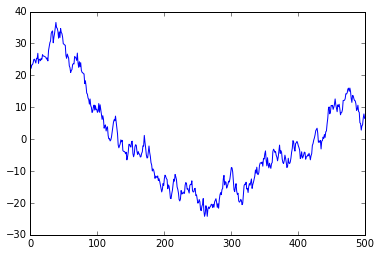
\includegraphics[width=\textwidth]{vis/random-process.png}}
	\label{fig:random-process}
\end{figure}

We then compare this random process to a real piece of market data.

\begin{figure}[H]
	\caption{Centered APPL stock price, some time after 2010}
	\centerline{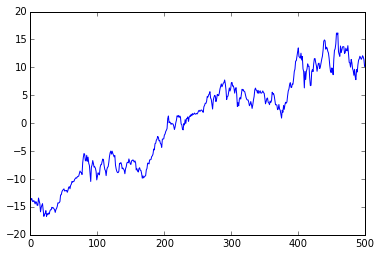
\includegraphics[width=\textwidth]{vis/appl.png}}
	\label{fig:appl-process}
\end{figure}

Presented with both of these diagrams, and without the aid of time scales or actual prices, most people would find it impossible to differentiate the diagrams. Using visual inspection alone, either of these diagrams could just as likely be a real piece of stock market data.

This gives us pause as there is little point in moving forward if the stock market is truly random and there is nothing to predict. However, this does not turn out to be the case. We will demonstrate that it is different to random in two ways. In the very next section, we will show that the price itself is fundamentally different to random data, and later we will show that the price is not as random as it may appear when take external variables into account.

\subsection{Quantitative Difference to Random pattern}

We will first show that the way in which markets move is fundamentally different to the way one would expect them to move if they were random.

\citet{karpio2007gain} describe an asymmetry between gains and losses on the stock market. Their research looks specifically at indices like the Dow Jones and how "you wait shorter time (on average) for loss of a given value than for gain of the same amount". However, this research was conducted in 2006, before the Great Recession. It is conceivable that the market conducts itself differently since then, and therefore we tried to replicate their findings.

On every day from the year 2000 to 2014, we simulated an investment on the Dow Jones index. We then counted the number of days it took for the investment to gain or lose 5\% of its original value. When it lost 5\% of its value, it was put into the red set, when it gained 5\% of its original value, it was put into the green set. The graph shows 2 overlaid histograms detailing how long it took for an investment to lose of gain 5\%.

\begin{figure}[H]
	\caption{Gain-Loss Asymmetry on the Dow Jones}
	\centerline{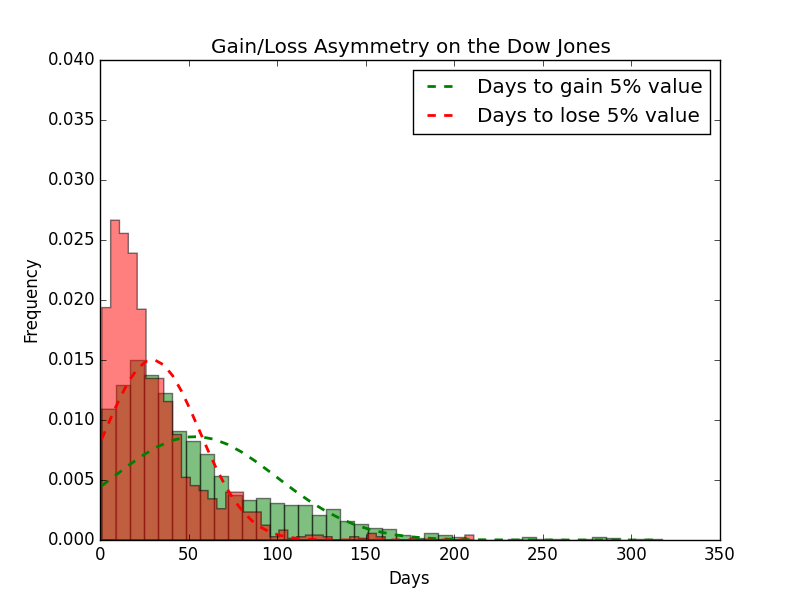
\includegraphics[width=\textwidth]{vis/gain_loss_asymmetry.png}}
	\label{fig:gain-loss-asymm}
\end{figure}

What this graph shows is that the market generally creeps upwards but is prone to sudden drops downwards, and supports the findings described earlier. This demonstrates that the stock market is fundamentally different to random data. This gives us hope for the remainder of the project. If the market price is not random, then it might be worth investigating and trying to predict.

\section{Efficient market hypothesis}

Another concept to keep in mind while working on the project, was the Efficient Market Hypothesis. Informally, the efficient market says that the market is efficient at finding the correct price for the stock market.

It comes in three flavors, however it is still a matter of debate which one, if any, are correct.

\begin{description}
  \item[Weak-form Efficient Market Hypothesis] 
  The weak form of the hypothesis says that no one can profit from the stock market by looking at trends and patterns within the price of a product itself. It is important to note that this does not rule out profiting from predictions of the price of a product based on data external to the price. We will see examples of prediction based on both in sample and out of sample data, and provide evidence in support of the weak form
  
  \item[Semi-Strong Efficient Market Hypothesis]
  The Semi strong form rules out all methods of prediction, except for insider trading. This means that if we are only to use public domain information in our prediction attempt, the Semi-Strong form says that we will be unsuccessful. Later in the project, we will provide results are seem to be inline with this hypothesis but not as good as with the weak form.
  
  \item[Strong form Efficient Market Hypothesis]
  The strong form says that no one can profit from predicting the market, not even insider traders.
\end{description}


Clearly, if we are to predict the stock market using only public information, we must hope that at most the weak form of the efficient market hypothesis is true so that at least then we can use external data to predict the price of a product.

\section{Self Defeating Strategies}

Finally there is the idea of a successful model ultimately leading to its own dimize. 

The insight is that if there were a simple predictive model that anyone could apply and profit from themselves, then over time all of the advantage will be traded and erroded away.

This is the same reason for the lack of academic papers on the topic of successfully predicting the market. If a successful model was made widely known, then it wouldn't take long until it wouldn't be successful any more.

\section{Conclusions}

The three preceding ideas ask us to keep an open mind on stock market prediction. It is possible that we will not be able to do it profitably.

\chapter{Attacking the problem - Fundamental Analysis}

The first approach we take at solving the problem of market prediction is to use Fundamental Analysis. This approach tries to find the true value of a company, and thus determine how much one share of that company should really be worth. The assumption then is that given enough time, the market will generally agree with your prediction and move to correct its error. If you determine the market has undervalued a company, then the market price should rise to correct this inefficiency, and conversely fall to correct the price of an overvalued company. 

\citet{graham1934security} laid the groundwork for the field with the book \textit{Security Analysis}. He encouraged would-be investors to estimate the intrinsic value of a stock before buying or selling based on trends, a novel idea at the time. It stands as testament to his approach that his only A+ student was Warren Buffet who methodically applied the strategy and has enjoyed renowned success since \cite{schroeder2008snowball}. This gives us some hope, but we should be cautious and remember that the economy might behave differently today than it did before.

It should be noted that Fundamental Analysis is compatible with the weak form of the efficient market hypothesis. As explained earlier, the weak form does not rule out prediction from data sources external to the price, which is what we will use to determine our fair market price.

We will look at two of the most common metrics used in fundamental analysis, Price to Earnings ratio, and Price to Book ratio to try and predict long term price movements on a year to year basis. This is the typical prediction range for Fundamental Analysis.

\section{Price to Earnings ratio}

The first metric for the value of a company that we will look at is the Price to Earnings ratio. The price to earnings ratio is calculated as

\begin{math}
  \\
	\text{P/E Ratio} = \dfrac{\text{Share Price}}{\text{Earnings Per Share}}
	\\
\end{math}

Roughly speaking, what this calculates is the price an investor is willing to pay for every \$1 of company earnings. If this ratio is high, it might be a sign of high investor confidence. If investor confidence is high, that might mean they expect high returns in the following year. We should then expect to see be a relationship between high P/E ratio and high returns in the following year.

To investigate this relationship, we plotted the P/E ratio for of 456 companies on the 31st of December against the change in stock price for the following year. We gathered these data points from the year 2000 to 2014. Below is a graph of this relationship.

\begin{figure}[H]
	\caption{Relationship between P/E Ratio and following year growth}
	\centerline{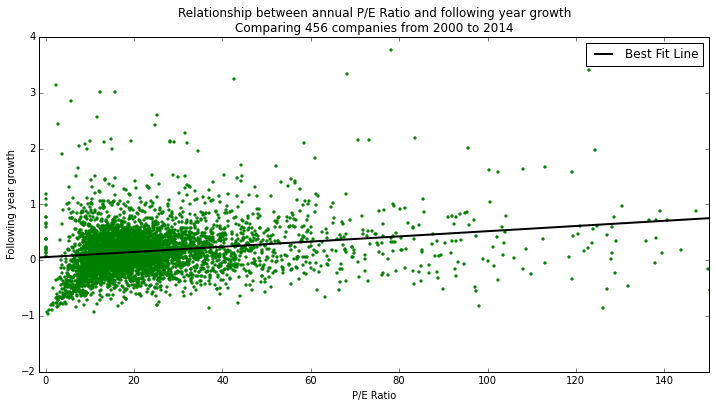
\includegraphics[width=\textwidth]{vis/pe-ratio-abs.png}}
	\label{fig:pe-abs}
\end{figure}

The best fit line was calculated using the standard Least Squares method. If the P/E ratio was indeed predictive, we might have expected a steeper slope in the best fit line, but we can see that there is a very weak correlation at best. It should also be noted that the more we remove outliers, the lower the slope becomes. This indicates that the the line is probably being pulled up by outliers rather than an actual correlation in the data. 

We can investigate the data further using a boxplot. Figure \ref{fig:pe-box} divides companies into two categories. The first category, $Gain\ Companies$, are companies whose share price increased in a given year, and the second category, $Loss\ Companies$, are companies whose share price fell in a given year. The box plot shows the distribution of P/E Ratios for each category.

\begin{figure}[H]
	\caption{Investigation of P/E Ratio predictive value using Box plot}
	\centerline{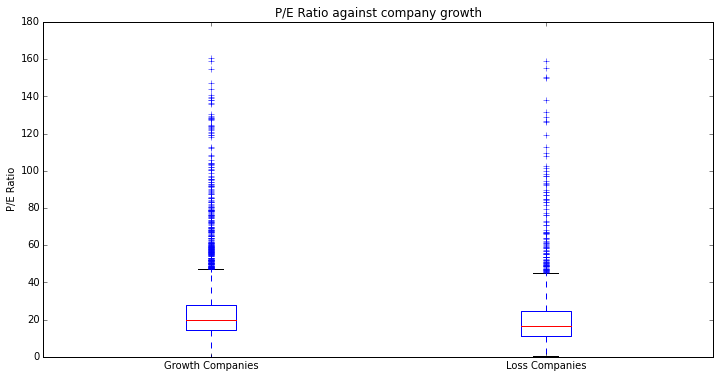
\includegraphics[width=\textwidth]{vis/pe_box.png}}
	\label{fig:pe-box}
\end{figure}

If the P/E Ratio was predictive, we would have expected a noticable difference in the P/E Ratio distribution of companies whose share increased, and those whose share price decreased. However, this is not the case. It is clear they the P/E Ratio distribution between these categories is almost identical. We can therefore conclude that the P/E Ratio has little or no predictive value when it comes to estimating company performance for the following year.

\section{Price to Book ratio}

The second metric for the value of a company that we will look at is the Price to Book ratio. The price to Book ratio is calculated as

\begin{math}
  \\
	\text{P/E Ratio} = \dfrac{\text{Share Price}}{\text{Book Value of Company}}
	\\
\end{math}

Informally, what this calculates is the ratio between the value of a company according to the market and the value of the company on paper. If the ratio is high, this might be a signal that the market has overvalued a company and the price may fall over time. Conversely if the ratio is low, that may signal that the market has undervalued the company and the price may rise over time. We should then expect to see a relationship between high P/B ratio and low returns in the following year. 

To investigate this relationship, we plotted the P/E ratio for of 316 companies on the 31st of December against the change in stock price for the following year. We gathered these data points from the year 2000 to 2014. Below is a graph of this relationship.

\begin{figure}[H]
	\caption{Relationship between P/B Ratio and following year growth}
	\centerline{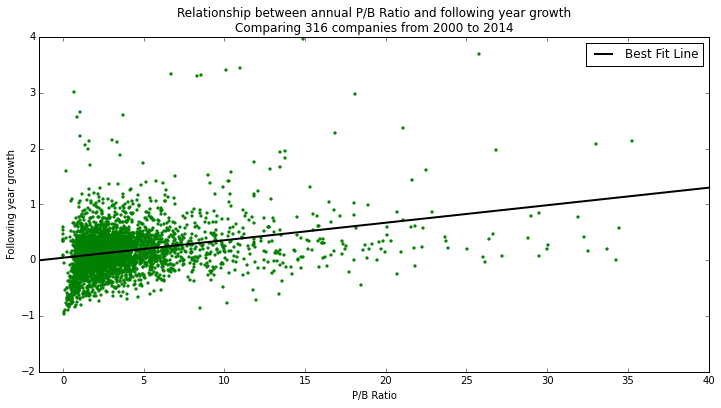
\includegraphics[width=\textwidth]{vis/pb-ratio-abs.png}}
	\label{fig:pb-abs}
\end{figure}

Just as in the P/B diagram, the best fit line was calculated using the standard Least Squares method. Although slope of the best fit line is greater than that of the P/E ratio, this is the opposite of what we might have expected. The data suggests that a high P/B ratio is somewhat  predictive of a high growth in the stock price. This is and unexpected result directly opposed to available literature on the subject \cite{jensen1997new}. 

One hypothesis is that a high P/B ratio could be a signal of investor confidence like the P/E Ratio and so might be able use the argument about how investor confidence could be a predictor of growth. More likely, we suspect, is that the data used does not control correctly for the expected growth in all companies over the studied time period, from 2000 to 2014. Even accounting for the Great Recession, the stock price of most companies in our dataset did grow from year to year. However, this does not fully explain why the slope of the P/B Ratio best fit line is greater than the slope of the P/E Ratio best fit line. One would have expected at least a lesser slope if the expected slope was an inverse relation. 

To better understand the predictive value of the P/B Ratio we can use a box plot. Figure \ref{fig:pb-box} divides companies into two categories, exactly as in the earlier P/E Ratio example. The box plot shows the distribution of P/B Ratios for each category.

\begin{figure}[H]
	\caption{Investigation of P/B Ratio predictive value using Box plot}
	\centerline{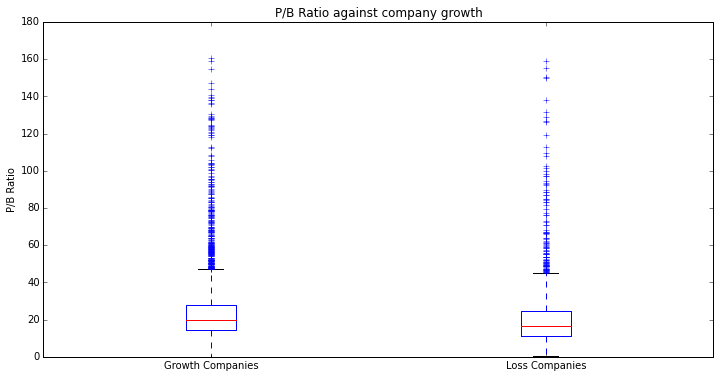
\includegraphics[width=\textwidth]{vis/pb_box.png}}
	\label{fig:pb-box}
\end{figure}

It is evident that this diagram tells a very similar story to the P/E Ratio diagram. We can see that companies that grew and companies that shrank had an almost identical distribution of P/B Ratios. If it were predictive, we would have expected different distributions for each category. We can therefore conclude that the P/B Ratio also has little or no predictive value when it comes to estimating company performance for the following year.

\section{Fundamental Analysis limitations}

There is an obvious pattern with fundamental Analysis. We are trying to find the quantify the true value of a company when almost every company has in some way or another some purely qualitative value

Fundamental Analysis methods does not attempt to capture, and so it difficult to build a software solution to do so. This leaves a large gap in knowledge an algorithm could learn about a company. How should it quantify the value of a brand, the size of its customer base, or a competitive advantage?

These are three examples of some of the many things that a human investor might take into account when deciding who to invest in, but they are untouchable within the scope of this project. 

Instead, we are limited to purely quantitative company metrics. We will look at two of the most common metrics, Price to Earnings ratio and Price to Book ratio.

\section{Fundamental Analysis - Conclustion}

We evaluated two Fundamental Analysis metrics and found no conclusive proof of their predictive value.  

These predictions are also very long term, looking one year into the future. Predictions on this time scale were not the focus of the project, instead we wanted to focus on predicting daily trends in the market.

Because of these issues that we moved away from Fundamental Analysis.

\chapter{Technical Analysis}


The second approach we take at solving the problem of market prediction is to use Technical Analysis. This approach tries to recurring patterns and trends within the price of the stock itself.

It should be noted that Technical Analysis goes directly against all forms of the efficient market hypothesis. As explained earlier, even the weak form of the hypothesis rules out prediction using historic price data alone.

Technical Analysis is used for daily level price prediction which was the original focus of this project. 

\section{Broad families of Technical Analysis models}

If a casual investor was to do some research into trading on the stock market using Technical Analysis they would encounter two broad categories of models. We will demonstrate that one of these is implausible in theory and in practice, while the other although sound in theory, does not work in practice.

\section{Naive trading patterns}

The first family of technical analysis methods we will look at are those that do not work in theory or in practice. These methods are based on looking for very high level patterns in the stock market price and using these patterns in an attempt to predict the following price movements.

Amoung the most common of these patterns is the Head and Shoulders pattern, and it is one of the worst offenders of poor methodology in the technical analysis of stock market field.

\begin{figure}[H]
	\caption{Head and Shoulders Pattern \cite{website:headshoulders}}
	\centerline{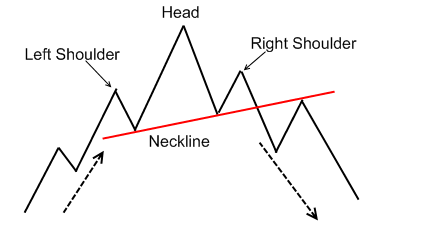
\includegraphics[width=\textwidth]{vis/headshoulders.png}}
	\label{fig:headshoulders}
\end{figure}

The diagram shows a bearish head and shoulders pattern. In this context, bearish is taken to mean falling share prices. The idea is that if a trader sees this pattern, they can expect the market price to then fall. To spot this pattern, a trader is supposed to look for two smaller peaks (the shoulders) surrounding a larger peak (the head). 

However, it can be shown that the pattern does not, and indeed cannot, provide useful information. 

The first issue is that the pattern cannot be identified until after it has happened. Not until the price falls away below the right shoulder, does it become apparent that a head and shoulders pattern has just occured. But this information needed to identify a the head and shoulders pattern is exactly what it was supposed to predict. This leaves no useful information for the trader. If the price were to rise after the right shoulder, it would not be a head and shoulders pattern. A common pattern here is that the investor does not see this as a case where the head and shoulders pattern failed, but instead a case where the head and shoulders pattern didn't exist. This is confirmation bias.

Because of the lack of theorethical support, it is easy to find many additional problems with the head and shoulders pattern. The most obvious one is that because we cannot identify the pattern until after the fact, we can never tell the way the market should move even if the pattern was predictive. Suppose we have observed a series market movements that appear to be similar to those in the diagram up to peak of the right shoulder. We have no way of telling whether the market will continue upwards, or follow the head and shoulders pattern downwards. If the pattern moved upwards when it was supposed to be at the right peak, the right peak could turn out to be a left should of another possible head and shoulders, or even a head peak.

In short, it is impossible to get any useful information from the head and shoulders pattern. However this does not appear to stop investors attempting to use it. A casual investor doing an internet search about trading patterns will more than likely bump into a blog post or an apparently authoritive source telling them how to use this pattern, or one like it, to profit on the market. 

There is no shortage of similar patterns to be found in online literature, but almost all fall into the same problems as the head and shoulders pattern. All information available from these models is only useful in retrospect. 

\section{Statistical trading patterns}

Next, we move to technical analysis models that are sound in theory. These models work on a statistical basis rather than patterns and make explicit predictions about the future. One of the simpliest and most common model of this type is the Moving Average Crossover strategy.

The moving average crossover strategy relies on the interaction between two moving average calculations. One is a short moving average, and the other is a long moving average. The short moving average might be the mean price for the last 10 days, and the long moving average might be the mean price for the last 20 days for example. When the short moving average crosses under the long, this can be intrepreted as a negative signal that the market is trending downwards. Conversely if the short moving average crosses over the long, this can be intrepreted as a positive signal that the market is trending upwards. The points at where these events happen are called the crossover points and can be categorised into negative and positive crossovers points.

\begin{figure}[H]
	\caption{Moving Average Crossover}
	\centerline{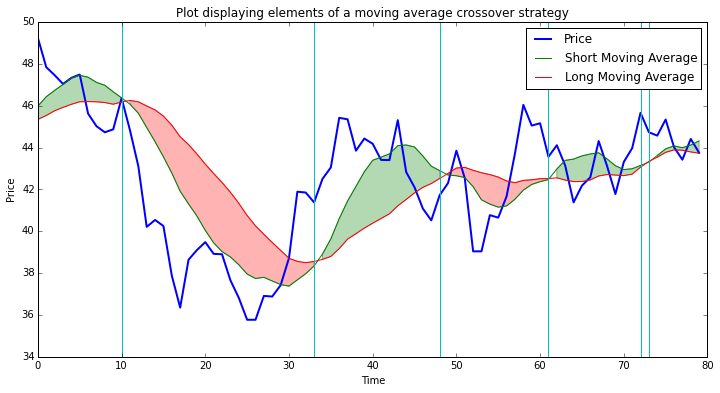
\includegraphics[width=\textwidth]{vis/macrossover.png}}
	\label{fig:macrossover}
\end{figure}

In figure \ref{fig:macrossover}, the red areas are where the short moving average is below the long moving average and the green areas are where the short moving average is above the long moving average. The diagram seems to give us hope for this strategy. The large green and red areas on the left of the diagram do indeed appear to be predictive of market upward and downward trends respectively. 

However, while it is attractive to look at the crossover points on the left of the diagram, one should not ignore the less significant crossover points on the right of the diagram. This are crossover points just as much as the ones on the left area but these are not as predictive for market trends. We need to choose a long and short periods moving average to maximize the predictive value.

\subsection{Evaluating the Moving Average Crossover model}

To evaluate the predictive value moving average crossover model, we attempted to build a predictor using these crossover signals (negative and positive) as the input features and the market trend for the following day as the dependent variable we are trying to predict. We performed a rigorous evaluation of long and short term pairs on a training set, and tested the winning long/short term pair against an independent test set.

To perform this analysis, assembled a database of daily prices of all 30 companies in the Dow Jones from the year 2000 to 2014.

This data was then augmented with $49$ new moving average columns. The first of these columns contained the 1-day moving average price, the second contained the 2-day moving average price, etc., up to the 50-day moving average price. This precomputation of the moving averages greater increased the time taken to train the model.

The data was split into a training and test set. For simplicity, we divided the data based on company. We chose 20 random companies and used them as the training set. The remaining 10 companies were used as a test set. This is similar to the single-holdout method, which under normal circumstances is not considered to be statistically credible. However there was sufficient data in this case for single-holdout to be viable. There were over 74,000 data points in the training set and over 38,000 in the test set.

The model itself was purposefully kept extremely simple so as to remain true to the intended usage of the moving average strategy. When a positive crossover occurred (short crosses over long), the model predicted the stock price would increase tomorrow, and when a negative crossover occurred it predicted the stock price would fall tomorrow. Deciding which long and short term periods to use can be seen as equivilent to finding the best hyperparameters for the model. This is model selection.

We perform a grid search over all possible long and short period pairs. For each period pair, we find the crossover the points between them. For each crossover point, we make a prediction based on its positivity or negativity, and compare tomorrows predicted trend against the actual trend. We can then calculate the accuracy of this short/long period pair and remember it if it is the best so far.

When we have iterated over all possible long and short pairs, we will have found the best period pair for predicting tomorrows trend in the training set. Table \ref{table:ma-test-results} displays the top 5 short and long period pairs and their test accuracy.


\begin{center}
    \begin{tabular}{l | l | l | l}
    Rank & Short Period & Long Period & Test set accuracy \\ \hline
    1 & 8 & 35 & 0.5229 \\ \hline
    2 & 8 & 34 & 0.5219 \\ \hline
    3 & 8 & 33 & 0.5127 \\ \hline
    4 & 2 & 37 & 0.5073 \\ \hline
    5 & 2 & 36 & 0.5016 
    \label{table:ma-test-results}
    \end{tabular}
\end{center}

The winning pair after model selection was $8$, and $35$ for the short and long period respectively. We then cross validated this against our test set. Our accuracy on the test set using the $8$, $35$ pair was 0.5157. This is slightly lower than our training score, as should be expected.

We can better understand what the model is doing by looking at the confusion matrix.

\begin{figure}[H]
	\caption{Cross-validation Confusion Matrix for Moving Average Strategy}
	\centerline{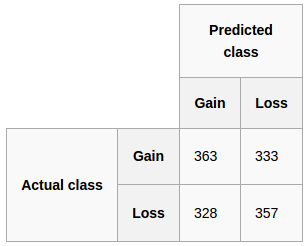
\includegraphics[scale=0.75]{vis/ma_confusion.png}}
	\label{fig:ma-confusion}
\end{figure}

We can now put into context how accurate the model is. We can see a slight increase in the numbers along the principle diagonal, indicating correct predictions. This gives us the slightly better than 0.5 accuracy score. But it is also obvious that the model isn't doing much better than a random predictor. We can quantify this using the Kappa Statistic, which compares the model's performance to a random version of itself based on the confusion matrix. This model scores a kappa of 0.0427, which is not significant. 

We must conclude that the Moving Average Crossover is not predictive in any meaningful way.

\subsection{Additional Technical Analysis Models}

[todo]

\section{Common problems with technical analysis}

For a casual investor, navigating online literature in this area poses a significant challenge. An extremely common theme in this literature is the poor methodology applied to evaluating trading patterns.

We have seen two examples of confirmation bias when we looked at the Head and Shoulders pattern and when we looked at Moving Average crossover points. In the former, patterns that didn't fit the narrative were simply ignored and in the latter people focused too heavily on the instances where it did work.

Even when there is no confirmation bias present, there is very rarely any proper separation of training and test set. Correct methodology would separate these examples so that one could accurately estimate how the model would perform given unseen examples, like it would have to do in the real world. This problem is prevalent when looking for short and long terms in moving average crossover. What many practitioners appear to do is find the best terms for their given time period and expect that to be just as predictive in future periods. This is incorrect methodology. You will always be able to overfit your model to preform well on a single piece of data, but this may not carry over to unseen examples.

Above, we applied the correct methodology. First we split the data into test and training sets, found the best term pair for the training set, and tested that on the test set. This gives us a true estimate of how our best estimator carries over to future data. This proper methodology is not common in online literature


\section{Technical Analysis - Conclusion}

It might have been expected that given the popularity of Technical Analysis for stock market trading, that there might have been a more positive result. However, somewhat surprisingly, the data shows that there is little predictive value to be found in Technical Analysis. 

\bibliography{report2}
\bibliographystyle{plainnat}

\end{document}
